\RequirePackage{snapshot}
\documentclass[10pt,twoside]{article}
\usepackage[sided=twoside]{tekfive}
\usepackage{float}
\usepackage{caption}
\usepackage{amssymb}
\usepackage{natbib}
\usepackage{tabulary}
\usepackage[scaled]{helvet}
\usepackage[absolute]{textpos}
\usepackage[left]{lineno}
\usepackage[yyyymmdd,hhmmss]{datetime}
\usepackage{comment}
\usepackage{xparse}

\ExplSyntaxOn
\NewDocumentCommand{\getenv}{om}
 {
  \sys_get_shell:nnN { kpsewhich ~ --var-value ~ #2 } { } \l_tmpa_tl
  \tl_trim_spaces:N \l_tmpa_tl
  \IfNoValueTF { #1 }
   {
    \tl_use:N \l_tmpa_tl
   }
   {
    \tl_set_eq:NN #1 \l_tmpa_tl
   }
 }
\ExplSyntaxOff


\renewcommand*\familydefault{\sfdefault}

\newenvironment{ppl}{\fontfamily{ppl}\selectfont\itshape}{\par}

\renewcommand{\abstractname}{Executive Summary}

\newcommand{\projectName}{\emph{AutonomousTrust }}
\newcommand{\analysisName}{\emph{Flexline }}

\bibliographystyle{unsrt}

\title{\textbf{\huge \projectName}\\ High-trust systems for secure cooperation}
\author{Sean M. Brennan}
\date{\monthname{} \the\year}

\begin{document}
	
\TekFiveTitle

\begin{abstract}
	Cybersecurity efforts are at a running-in-place standstill due to the utterly non-scalable assumptions currently embedded in our computing paradigms.
	Software, hardware and administrative strategies, too numerous to count, all attempt to shoehorn security into new and existing systems, only to impair automated cooperation and collaboration.
	We struggle with this because default human models of reciprocity simply do not hold at large scales, or when participants are at cross-purposes.
	Our software constructs unconsciously reflect that.
	
	We should not have to think about security, automation should take care of that for us.
	Why doesn't it?
	Because we haven't taught computers how to trust.
	To combat this limitation we allow the machine to be in charge of the trust model - and that in turn unlocks more efficient processing (less noise), more direct routing (no middleman), and as such much greater scaling, securely.
		
	The ecosystem we present here is fully realizable with current technology --- no special hardware (though we might be careful about what we choose), no unproven libraries (but again choosing carefully) --- just small XML messages over any connection and a few small, shared blockchain ledgers.
\end{abstract}

\getenv[\SCENARIO]{AUTONOMOUSTRUST_SCENARIO}\show\SCENARIO

\section{Introduction}\label{sec:intro}
When the Internet was young (ARPA-net and into the BBS-era), participants were necessarily specialists, and existing social controls allowed for fine-grained trust calibration.
The Internet rapidly advanced well beyond that state, but we continue to act as if human social techniques -- evolved for relatively small groups -- are adequate for an extremely large-scale environment.
In the Cloud, we run proprietary processes with highly sensitive data on someone else's hardware and struggle with the opposing demands to maintain control of access yet be productive in a timely manner.
Zero Trust may be just a re-packaging of well-known system security best-practices (individualized credentials, least privilege access, time-limited sessions) but it is indicative of the growing network security crisis that is already upon us --- and that our best answers are over thirty years old.
Clearly the current cybersecurity paradigm is in trouble: ever-increasing restrictions are complex and anti-scalable, and have but one logical end-point - total lockdown of all resources.
This is the opposite of what we want.
\\[10pt]
What do we want, ideally?
In very general terms, as an owner of certain resources, I want to only give access to the extent that I benefit, no more, no less.
As a user, I also want to benefit from that access, and, aware or it or not, I have value to offer the resource-owner.
Whether client-server or peer-to-peer, every external computation or data-exchange is an implied contract, with risks as well as rewards, along with an implicit level of trust.
So let's make all that \emph{explicit}.

Our premise is that system knowledge -- particularly security context -- is local, situational, and ever changing.
It is best then if control, detection and response are also local.
It follows that we must embrace automation to recreate trust structures for data-sharing.
Like many other successful computing paradigms (genetic algorithms, swarm optimization, neural networks), a solution to this problem becomes apparent through modeling biological processes, in this case, human trust.
What do human trust relationships look like?
\\Generically, they:
\begin{enumerate}
	\item are \textbf{scalable}, multilayered in small groups, allowing a broad but shallow hierarchy, most clearly in military, government or corporate organizations; \label{scale}
	\item share \textbf{language}, often exclusive to a community -- linguistic constructs act as in-group signifiers in addition to means for more efficient knowledge-transfer; \label{language}
	\item share \textbf{goals}, concerns, beliefs or mission; \label{mission}
	\item require \textbf{consistent identity} (preferably immutable) -- naturally accomplished by face-to-face interactions; \label{identity}
	\item are \textbf{reputation-based}, using dynamic evidence of intent -- a lifetime to build, seconds to destroy; \label{reputation}
	\item are \textbf{optimized} in the case of strangers interacting where reputation information is sparse (e.g.\ two-strikes rule); \label{optimized}
	\item are \textbf{prioritized}, utilizing shortcuts, frequently in the form of social roles, since tracking trust relationships tends to be high cognitive load. \label{priorities}
\end{enumerate}
We will justify our breakdown of trust relationships into these seven facets in section~\ref{subsec:trust}.
\\[10pt]
Machine trust would be built with similar characteristics (respectively):
\begin{enumerate}
	\item limited direct communication among peers, but with hierarchical network traversal;
	\item a domain-specific markup language descended from an ur-language, easily extended -- the language a machine implements indicates the groups it participates in;
	\item a strict negotiation protocol, reaching accord in agreed goals;
	\item a crypto-ledger for identity, shared directly among cohorts only but accessible as sub-chains anywhere;
	\item transaction outcome evaluation/scoring, shared and self-immutable -- machine reputation is both public knowledge yet privately evaluated;
	\item allows onboarding and reputation bootstrapping through game-theoretic strategies;
	\item assuming scalability (\#\ref{scale}) is optimized, various prioritization strategies (gullibility, cynicism) can be employed to balance opportunity versus security in groupings that include strangers.
\end{enumerate}
Note that the machine characteristics above directly implement the corresponding aspects of the human trust model.
This reveals our founding assumption: that human trust mechanisms, developed over at least one hundred thousand years, is likely to be more effective than anything we can design.
This is detailed in section~\ref{sec:implementation}.


\subsection{Concept}\label{subsec:concept}

\textbf{\projectName}is TekFive's high-trust cooperative computing concept --- a data messaging framework that allows for dynamic composibility, requesting and serving encrypted data \textit{only} with trusted peers and only to the extent of that fine-grained trust.
Said trust is dynamically evaluated in real time to rapidly eliminate incoming threats and even reclassify existing peers as their behavior changes and thus protect resources.
Greater risk requires greater trust.
An autonomous agent using this framework can adaptively: 1) refuse communications from severely untrusted peers, conserving bandwidth; 2) communicate with but refuse computation services to faintly trusted peers, protecting CPU time; 3) offer services but refuse data-sharing to moderately trusted peers, protecting data; \textit{and} 4) offer data-sharing to well trusted peers; all with a configurable gradient of access at every level, and all within the same application.

In more concrete terms, \projectName is an operations framework for a vast distributed system that dynamically composes numerous individual micro-services into a coherent application on-demand -- with security at its core.
We follow the Unix philosophy: do one thing well, work together, use a universal (text) interface; yet implemented such that each micro-service can choose it's level of participation.

To illustrate this concept in detail, we will describe a use-case involving secure data-sharing among several entities.
Within this example, we discuss the above seven system facets of communication, language, negotiation, identity, reputation, optimization and prioritization.
Orthogonal to, and cutting through, these conceptual divisions, yet also of critical importance, are operational concerns such as sub-system management and debugging, service discovery, dynamic name-to-address mapping, network resiliency and message reliability.


\section{Background}\label{sec:background}
Wherein we review the literature on the relevant state-of-the-art for human trust relationship modeling, automated machine communication, reputation systems, and cybersecurity.

\subsection{Human trust models}\label{subsec:trust}

The state of the art in understanding human trust (interpersonal trust in the social literature) is rather amorphous, suffers from foundational issues of taxonomy, and formal formulations of the mechanics of trust are almost non-existent.
Therefore, we will be connecting the dots to span gaps in the social and psychological literature.
Our simplified human trust model outlined above is based on discoveries in evolutionary biology and experimental economics as related to self-enforcing game theory and reciprocity.
\\[10pt]
The limits of personal social scale (\#\ref{scale} of our model) are well explored in Dunbar, giving us a ranged maximum of around 100 to 230 peers (often the number 150 is used as short-hand for this range)~\cite{dunbar1992neocortex}.
This number is subject to community cohesion and mission urgency, such that less of either results in a smaller maximum scale.
Additionally, human groups have tiered scaling at membership numbers at 5, 15, and 35 individuals for progressively less intense relationships~\cite{hill2003social}.
These numbers also demonstrate the cognitive limits inherent in social reach, with direct implications for trust.
In a military setting, the maximum limit is roughly the size of a company and the minimum that of a squad, but an overarching hierarchy of larger-than-maximum structures is used to loosely cohere the whole.

Language (\#\ref{language}) is a critical bonding element in human socialization, partially fulfilling the same social role as grooming in other primates~\cite{dunbar2004gossip}.
As such, this permits bonding and collaboration across temporal and spatial distance, and additionally over a larger scale of participants.
Dunbar notes that language is used for knowledge-passing, behavior-policing, self-promotion, and deception; all of which fold directly into the nature of trust relationships.

Shared goals (\#\ref{mission}) contribute greatly to collective coherence and are observable in nonverbal human behavior, separating merely working nearby another from working together~\cite{sacheli2015social}.
Notably trust is hardly present or needed in the latter, but critical for the former.

The importance of consistent personal identity (\#\ref{identity}) in human social interaction is a major gap in the literature.
As humans, we assume (inaccurately) that individual identification of our social peers is correct, and it usually is, but at the extremities of the Dunbar number perhaps not so much.
That this \emph{can} happen at all is seen from the social reaction to inconsistency.
Revealing false identity, misrepresentation, or mis-identification results in immediate distrust, manifesting in emotion ranging from embarrassment to aggression.
The social impact of this is so strong that we are sensitive to our own presentation: consistency of self-identity directly relates to psychological well-being~\cite{suh2002culture}.


Reputation (\#\ref{reputation}) enables indirect reciprocity, i.e.\ an actor reacts to a peer based on how it is likely to affect their reputation with 3rd parties, rather than the immediate interaction~\cite{phelps2012emergence}.
Despite high dynamism in individual reputation status, overall human social network metrics tend to equilibrium.
Both indirect and direct reciprocity are the bases of trust relationships.

To determine approaches to optimization (\#\ref{optimized}) for direct reciprocity, separate from cooperative reputation strategies, we turn to game theory.
Axelrod's generous or contrite tit-for-tat (TFT) has been consistently shown to disarm the always-defect tactic, making space for fragile but more optimal and stable strategies such as win-stay/lose-shift~\cite{axelrod1981evolution, axelrod1997complexity, nowak1995arithmetics}.
In an iterative prisoner's dilemma game, TFT is a strategy wherein an actor cooperates until the other defects, then defects until the other cooperates.
The generous (GTFT) and contrite (CTFT) variants either cooperate more often or defect less often (respectively), and they do somewhat better than plain TFT. This effectively ensures a non-zero-sum game.
Win-stay/lose-shift (WS/LS) is an approach wherein an actor only swaps cooperation or defection upon losing a round, but otherwise sticks with what worked previously.
WS/LS is vulnerable to always-defect (as all strategies but TFT are), and so needs the guard-dog of TFT to keep it safe.

Prioritization and shortcuts (\#\ref{priorities}) are critical because processing social network information can be cognitively taxing and thus place limits on social group scales~\cite{davidbarrett2013processing}.
As an example, hierarchical social structures are a frequent means of bypassing this limitation, but still utilizes heuristics for rapid in-group identification.
This means as scale grows, social roles play a greater part of trust structures.


\subsection{Distributed machine-to-machine communications}\label{subsec:m2m}

A precursor to the message-sharing aspect of the system described herein was articulated by Vestrand, et al.\ as the Dynamic Coalition Architecture (DCA), implemented as the Python SatChat library~\cite{vestrand2021artificial}.
Originally applied in the astronomy community - socially a small, well-connected group of scientists with relatively high cohesion - SatChat enabled rapid, controlled sharing of global telescopic data to enhance automated rapid response to detections of extraterrestrial events.
It utilizes a published XML schema which dictates an open message header and an encrypted body, a centralized routing process, and simple communication via zeroMQ that assumes a reliable substrate.
This DCA system worked well in it's intended environment.
In an effort to expand funding, DCA was then applied to a very different environment: coordinating sensory data and model conclusions among six national laboratories.
DCA did \textit{not} do well.
The human-social assumptions no longer held and in fact exhibited negative cohesion, and the software itself was (naturally) unable to compensate. \projectName tackles that challenge of interpersonal distrust head-on, but shares zero intellectual property with Vestrand's library.

More generally, machine-to-machine communication (M2M) consists of automated message-passing and coordination driven by artificial intelligence (AI), machine learning (ML), or simple command-and-response scripting.
M2M can be found in telemedicine, mobile payment (Google Wallet/Apple Pay), smart home systems, or the amorphous internet of things (IoT). As an example, a prominent protocol (and ISO recommendation) for M2M is Message Queuing Telemetry Transport (MQTT), providing a publish/subscribe transport.
Much like SatChat/DCA, it relies on a central broker server to route and distribute messages between resource-constrained clients using low overhead and allowing high latency~\cite{oasis2019mqtt}.


\subsection{Reputation-based systems}\label{subsec:reputation}

When reviewing the literature for machine reputation, it is important to distinguish whose reputation.
Online Reputation Management (ORM) is a very active field that focuses on business and user reputations.
It is human-oriented and thus unrelated to this work, though it may look similar in its toolset~\cite{hasan2022privacy}.

The most relevant field for our purposes is frequently part of Multi-Agent Systems (MAS) or Distributed Artificial intelligence (DAI).
Per a meta-review of the multi-agent literature by Granatyr, et al., other work on computational trust and reputation consists largely of theoretical and/or academic models~\cite{granatyr2015trust}.
In contrast to \emph{all} the 106 models surveyed therein, \projectName is not domain-specific.
Our work does fall under their numeric paradigm, as opposed to their cognitive paradigm (wherein agents reason about trust), but does not use statistical methods as ``almost all'' others do.

Notably, despite massive interest and dire need, no product has emerged out of academe.


\subsection{Cybersecurity}\label{subsec:cyber}

In this section, we distinguish between compile-time security (software design and vulnerabilities) and run-time security (access control, threat detection).
Compile-time vulnerabilities are always a class of insider threat (innocent or malicious), whether it be backdoors, trojan horses, spoofing, or simply exploitable bugs.
Much of what appears to be run-time attacks is only possible through compile-time (or configuration-time) vulnerabilities.
For example, malware is powerless if the operating system refuses to run it.
Man-in-the-middle (MITM) attacks can do nothing with strongly encrypted end-to-end communications.
If software development, installation, and use (such as password practices) are all on-point, then the available attack surface of a system is greatly minimized.

True run-time vulnerability then consists of attacks such as denial-of-service (DoS and DDoS), direct access and tampering, and social engineering.
These are all attack vectors that cannot be sealed off a-priori.

Current cybersecurity techniques for mitigating these threats largely consists of Blue-team response to Red-team hacking.
Most solutions passively seek to cut off attack vectors (firewalls, disk encryption, authentication, least-privilege).
Such policy-based protections are currently marketed as Zero-Trust Architectures.
Active solutions usually involve vulnerability detection (proactive), intrusion or anomaly detection (reactive) and postmortem forensics~\cite{anderson2020security, brooks2018cybersecurity, wittkop2022cybersecurity}.
Combining all of these approaches represents the industry-best-practice of defense-in-depth.

\projectName focuses on run-time threats, but also acknowledges that compile-time discipline and vulnerability monitoring are critical (see Section~\ref{sec:vectors}).

\section{Implementation}\label{sec:implementation}
Wherein we explicate precisely the what, the how, and the why of \projectName.

\subsection{Exemplar use-case}\label{subsec:use}

To better elucidate our system concept, we posit \input{scenario_\SCENARIO_setup}

\begin{ppl}
Offset by text that looks like this paragraph, the following sections show how each of the seven facets mentioned above in section~\ref{sec:intro} contribute to this use-case.
\input{scenario_\SCENARIO_0}
\end{ppl}

\subsection{Communication and messaging}\label{subsec:comms}

In addressing model facet \#\ref{scale} (scale), we note that decentralization is critical to scalability, therefore we utilize peer-to-peer direct messaging.
Address-lookup for directly-unknown resources is handled by the network hierarchy.
Similarly, we are carrier and protocol agnostic.
All communications use cryptography from end to end.  % post-quantum elliptic-curve crypto
What all this means in practice: NNG messaging written in C, Curve25519 key exchange with ChaCha20-Poly1305 transport cipher, and a custom replacement for the Domain Name System (DNS) (see section~\ref{subsec:id}).
These details allow us to make messaging itself a first-class trust-scoreable transaction, which in turn leads to the ability to dynamically tune-out harmful messaging with our trust mechanism.
Deliverability reports trace message receipts to determine underlying network reachability at any given time, which can be critical if the application requires timeliness or reliability.

The network hierarchy is neither imposed nor static, but rather dynamic and emergent.
Figure~\ref{fig:network} shows an example connection topology.
More highly-connected, resource-rich nodes become natural peer leaders serving as a clearinghouse for message schema.
They also coordinate with higher levels of the hierarchy for service discovery and identity propagation.
Branches of the hierarchy may grow or shrink, and peer leaders may rise or fall in accord with their capabilities.
At all times the trust mechanism is also in play, and will affect the structure of individual enclaves.
All hierarchy leaders are also participants in their own enclave, so the network graph will not look like a strict tree.

\begin{figure}
	\centering
	\includegraphics[width=0.4\linewidth]{network}
	\caption{Sample network connectivity graph}
	\label{fig:network}
\end{figure}


The next step is having a common language (facet \#\ref{language}). We use inheritable, extendable XML message formats (both human and machine readable), with an open and universal header while everything else is encrypted.
After the short, in-the-clear addressing header, a domain typology subheader which describes the message schema (like an email subject line) allows for rapid discard of unwanted messages.
Since decryption is streamed (using the transport cipher), connections can be cut early, reducing the harm from DoS attacks.

Finally, to established shared goals (\#\ref{mission}), domain-specific XML schema, nested into the generic format, define how specific data are exchanged.
A single communication agent can support a number of schemas.
Thanks to these schemas' specificity, messages can be kept short and efficient.

\begin{ppl}
\input{scenario_\SCENARIO_1-3}
\end{ppl}


\subsection{Identity}\label{subsec:id}

It is vitally important for agents in this system to be able to uniquely and immutably identify others (\#\ref{identity} from our model).
To this end, peer-level identities are recorded in a distributed crypto-ledger as a blockchain.
An identity record consists of a unique string, a crypto-signature, a public key, a timestamp (for update consistency), and an IP or MAC address for routing (see Table~\ref{tab:identity}).
A node can change its own address field in the ledger (subject to verification by peers), but no other fields --- short of starting from scratch and creating a new identity.
As we shall see, starting over has its cost.

\begin{table}[h!]
	\centering
	\begin{tabular}{ |l||c|c|c|c|c| }
		\hline
		& UUID & signature & public key & timestamp & routable address \\
		\hline
		bytes & 16 & 64 & 32 & 8 & 16 \\
		\hline
	\end{tabular}
	\caption{Identity record}
	\label{tab:identity}
\end{table}

Peer leaders (i.e.\ a or the link up the hierarchy) coordinate the local identity blockchain as a subchain on the next level of the hierarchy.
The global identity ledger is therefore a directed acyclic graph (DAG), also known as a blockdag.
Instead of an unwieldy monolithic entity, the overall identity blockdag is really a collection of pointers to subchains, all of which live at the peer level.
Note that the dynamic nature of the hierarchy means that any peer node can (and must be able to) adopt any hierarchical role.

\begin{ppl}
\input{scenario_\SCENARIO_4}
\end{ppl}


\subsection{Negotiation and trust-building}\label{subsec:negotiation}

The core of \projectName is a mechanism for indirect reciprocity in the form of reputation (model facet \#\ref{reputation}).
Transaction scores that contribute to reputation are stored in another blockchain separate from identity.
A transaction record consists of a unique identifier, a timestamp, and id, score and signature for each of the two transaction participants.
As with identity, reputation ledgers are subchained throughout the network hierarchy.
Tracking raw transaction scores allows agents to weight those scores based on the reputation of those doing the scoring.
In other words if an agent trusts A more than B, it will also trust others that A rates highly.

\begin{table}[h!]
	\centering
	\begin{tabular}{ |l||c|c|c|c|c|c|c|c|c| }
		\hline
		& UUID & type & timestamp & A's UUID  & A's score (of B) & A's sig & B's UUID &  B's score (of A) & B's sig \\
		\hline
		bytes & 16 & 4 & 8 & 16 & 8 & 64 & 16 & 8 & 64 \\
		\hline
	\end{tabular}
	\caption{Transaction record}
	\label{tab:reputation}
\end{table}

A word about blockchain consensus (aka Distribute Ledger Technology [DLT]): to achieve distributed agreement in the face of malicious participants (known as Byzantine failure), blockchain algorithms either assume that all participants are known (Byzantine Paxos, PBFT), or not known (Proof-of-Work, Proof-of-Stake, Proof-of-Authority, etc.).
\projectName has both cases.
The identity blockchain must presume initially unknown participants, but updates are infrequent.
The reputation blockchain \underline{must} know all participants, and updates very frequently.
We therefore use different algorithms for these different cases as appropriate.
%Proof-of-Authority (PoA) is a blockchain consensus approach that utilizes reputation

As noted previously, messaging is itself a reputation-impacting transaction.
This means that in a busy network, computing reputation from raw transaction scores can be very computationally intensive.
Therefore, agents keep a local, private data structure that facilitates fast reputation queries and updates as new transaction records come in.
Well-trusted peers can directly gossip, providing pre-computed reputation scores to others.

Reputation therefore represents an inversion of risk.
All requests for services, be it computation or data, must be negotiated as specified in communications schema, and reputation plays a large part.
A transaction client weighs the risk of a low-reputation provider against its need for the service.
In turn, the service provider weighs the risk of a low-reputation client against the resource exposure requested and the reciprocity value that the client brings.

\begin{ppl}
\input{scenario_\SCENARIO_5}
\end{ppl}


\subsection{Data evaluation and decision-making}\label{subsec:eval}

Transactions are scored on transparent, schema-defined or negotiated criteria, usually in terms of result applicability and timeliness.
Likewise, service providers can rate a client on their adherence to negotiated terms.
Because results must be validated, transaction record submission may be delayed, but bounds for this delay are also a agreed-upon criteria.
The validation decision is automated --- which implies some kind of adaptive facility such as AI. Inability to validate in a timely manner is a failure and affects reputation.
This may be outside of the control of a participating agent, so reputation is nuanced with transaction types to give the system better flexibility to deal fairly with low-resource or poorly connected (or overly ambitious) peers.

When bootstrapping new peers (or the system itself), there is no reputation information.
In this case, or in the case of coordinated attack, \projectName degrades to a minimal optimization mode (\#\ref{optimized} of the model).
Without a foundation of reputation to rely on, the system initially uses CTFT (see Section~\ref{subsec:trust}), then WS/LS to establish a reputation density threshold.
When onboarding a new peer, only that peer is targeted for this behavior.
Also when established reputation levels are too low (indicating either widespread hardware problems, network capacity overload, or malicious activity), the system likewise reverts to this mode to rapidly find and eliminate bad actors and trouble spots.
Note that this may lead to a virtual version of the dreaded network partition, making some valid agents, especially up the hierarchy, unreachable.

\begin{ppl}
\input{scenario_\SCENARIO_6}
\end{ppl}


\subsection{System administration and extension}\label{subsec:admin}

It sometimes seems that the only way to be secure is to be isolated, maximally partitioning the network.
This is illusory, and as we shall see in section~\ref{sec:vectors}, is an attack vector.
The reality is that system peers need to balance the priorities (facet \#\ref{priorities}) of security against seeking `social' opportunities, connecting to agents outside the enclave --- as secondary contacts in contrast to primary, domain-driven interactions.
These service discovery mechanisms are also what create the domain-enclave in the first place.

At any given time, agents can act as a client or as a server, requesting services or offering them.
At the peer level, there is no centralized yellow-pages-style listing.
In a client role, agents can announce a domain interest.
Otherwise, in server roles, they can advertise their services.
These messages are collated by peer leaders in order to efficiently traverse the hierarchy.
This encourages cross-domain communications and system-wide trust versus clique-formation.

\begin{figure}
	\centering
	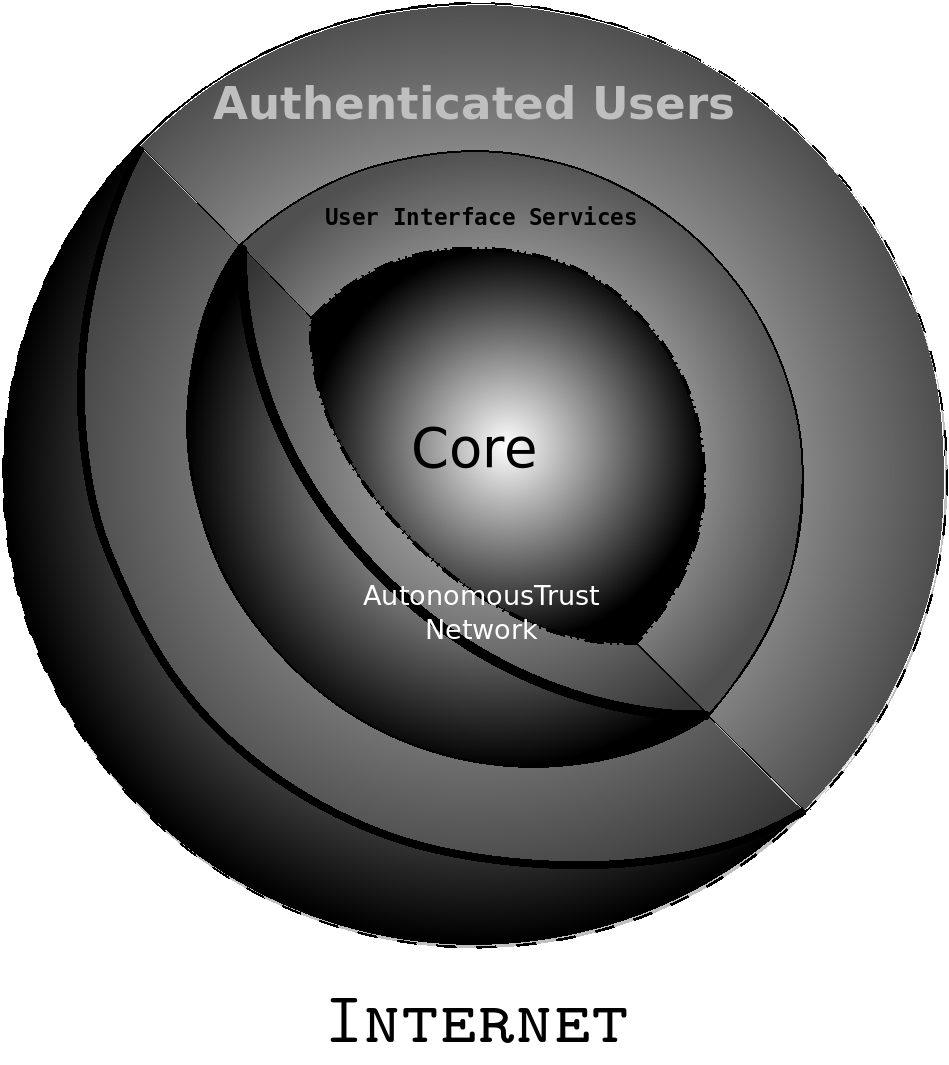
\includegraphics[width=0.4\linewidth]{users}
	\caption{User interfaces}
	\label{fig:users}
\end{figure}

Outside of the programming phase where agent capabilities are defined, user interaction with agents is strictly based on configuration (new schemas or negotiation inputs) or triggering events such as functionality or data requests, or authorizing new networks.
Users are kept in a domain separate from the main activity of the network, as seen in Figure~\ref{fig:users}.
This is a key aspect of system security, similar to CPU protection rings which restrict direct hardware access.
This clearly becomes a challenge for debugging or simply administering a system, likely solved by administrative agents.

\begin{ppl}
\input{scenario_\SCENARIO_7}
\end{ppl}

\section{Security}\label{sec:vectors}
This system is for naught if it does not protect against attack.
To get a sense of how \projectName might fare against real-world conditions, we consider the novel 2019--20 SunBurst software supply chain attack via the SolarWinds Orion network administration tool.
Analysis of this attack suggests that, aside from the initial SolarWinds network breach, state-of-the-art cybersecurity techniques and tools would have been ineffective at preventing or even detecting this hack~\cite{gao2022cybersecurity, fireeye2020sunburst}.
Once inside the network, attacker activity would have been indistinguishable from that of valid developers, and client companies would have no reason to cut-off Orion's access to the Internet.
In short, while Zero-Trust would have likely prevented the initial network hack, neither it nor most intrusion detection systems could have halted the rest of this attack.
Notably, Ken Thompson predicted and even wrote an implementation of this attack style, and commented on the almost total inability to detect it four decades ago~\cite{thompson1984trust}.
With either social engineering or other insider access, instead of just a possible lousy password, a repeat of this attack is currently unstoppable.
And how would you ever know that a more sophisticated version of this attack isn't already humming along inside your network already?

\projectName makes this attack \emph{impossible}.
Using our system, even code developers would not have direct access to the build system -- eliminating the binary injection.
Clients that used an \projectName-based product would immediately know if that product was violating the scope of its specification, when the Trojan Horse either phones home or tries to control the rest of the client system.

As mentioned in section~\ref{subsec:cyber}, compile-time security is outside the scope of this system --- but that does not mean we will ignore it.
Such security is a well-understood problem, although it can become complicated as a code-base grows.
In an over-simplified nutshell, it consists of careful design with correct implementation, and vigilant monitoring for vulnerabilities coupled with rapid mitigation.
TekFive offers products and techniques that address these problems, which we use in implementation -- specifically our \analysisName vulnerability discovery product and our code-correctness proofing expertise.

Run-time threats, however, are fundamentally complex and this emerges at large scale.
As this is a new computing paradigm, some attack vectors are solved by the nature of the system, some explicitly by design.
Such are fairly obviously no longer problems.
Some means of attack, particularly known distributed computing weaknesses, require research into the resiliency of our system to demonstrate its resistance.

\subsection{Possibly solved}\label{subsec:possibly-solved}

We believe the following known attack vectors are either significantly or wholly ameliorated (and this must be confirmed):

Because every message is encrypted end-to-end with post-quantum techniques, classic identity attacks (MITM, spoofing) are neutralized.

Although metadata attacks (who associates with whom) are hampered by only exposing identity/address pairs in messaging, they are still possible.
This system allows for near-contact networking with long latencies, so due diligence could eliminate the collection of metadata also.
Additionally, identities can be anonymous and still be useful --- at least in domains that do not demand KYC (know your customer).
Such anonymity renders metadata harvesting mostly useless.

DoS is largely mitigated by rejecting spurious messages, but at large enough scale can continue to be a problem until and unless network switches themselves run this system also.
With firmware-level enforcement, DoS can be eliminated and even the impact of DDoS can be lessened.

DLT-specific attacks that attempt to inject bad blocks into the chain, such as DDoS or the 51\% attack, are significantly reduced by our use of two disparate but mutually supporting blockchains and the required investment of reputation-building.


\subsection{System-specific}\label{subsec:system-specific}

The foremost class of attacks this system is susceptible to is divide-and-conquer tactics facilitated by \textit{lying}.
The solution in every case is to uncover the lie, then respond with the warhead of TFT, but such detection is not always easy.

Firstly, there is straight-up \textbf{Deceit}: malicious agents may falsify data or results.
In \projectName, this cannot survive when competing service providers are present.
Even a single client can make comparisons that will reveal this attack.

Next we have the case where a peer builds trust up just to betray it.
The \textbf{Frenemy} is a singular malicious agent that is patient enough to choose its time to strike.
Such a strike is very costly as it must be public, and as such can only occur once for a given identity.

In \textbf{bad reputation}, a group of peers colludes to drive your agent's reputation score down, most easily through gossip, but also via low transaction scores.
A peer leader can independently review and verify gossip in the former, and for the latter case can increase your external connections to test if your agent is the problem.

The infamous \textbf{Sybil} attack occurs when numerous agent identities controlled by a single entity seek to interfere with or derail the network.
The textbook solution to this is to make identity generation expensive. \projectName identities are cheap to create, but reputation is hard-earned.
Impatient Sybils are trivial to ignore.
Sybil Frenemies however are a serious threat.

\textbf{Atomization}, known in distributed computing as the Eclipse attack, occurs when malicious agents isolate a given peer.
This is often also a Sybil attack.
The isolated agent may be unaware that the data and reputations it is seeing is false.
This can be mitigated by having connections outside the enclave.

\textbf{Wicked Captain} is atomization caused by an authority in the hierarchy.
An entire enclave can be affected by this, but as any peer can become a leader, out-competing a malicious authority is an easy fix.

\section{Conclusion}\label{sec:conclusion}

\projectName represents a new paradigm in computing wherein security is \underline{primary}.
Combining the best of cryptography, blockchain, and distributed computing technologies, this system creates a setting for automated software agents to interact and self-regulate as a community.
When combined with TekFive's \analysisName product and program-correctness expertise, \projectName offers a comprehensive environment for decentralized computing that minimizes security risks and optimizes cooperation.
\\[10pt]
\input{scenario_\SCENARIO_conclusion}
\\[10pt]
One glaring omission we have not addressed here is the potential vulnerabilities presented by the operating system and hardware that \projectName runs on.
The equally obvious solution would be to run our system on bare metal, or a minimal, provably-secure OS. This will be the subject of additional research.

\bibliography{HighTrust}

\end{document}
